\documentclass[11pt]{article}
\usepackage[margin=1in]{geometry}
\usepackage{graphicx,amsmath,amssymb,booktabs,hyperref,xcolor,authblk}
\usepackage[numbers,sort&compress]{natbib}
\hypersetup{colorlinks=true,linkcolor=blue,citecolor=blue,urlcolor=blue}

% ---- numbers emitted by paper/experiments.py (results.json); set once here ----
\newcommand{\Popt}{0.63}          % P(optimum) at p=2
\newcommand{\Conc}{10.0}          % concentration over uniform (x)
\newcommand{\AR}{0.92}            % approximation ratio at p=2
\newcommand{\ARd}{0.93}           % approximation ratio at p=4
\newcommand{\Poptd}{0.75}         % P(optimum) at p=4
\newcommand{\Puniform}{0.0625}    % 1/2^n
\newcommand{\TailErr}{0.07}       % IQAE tail-prob relative error (%)

\title{\textbf{Watching Language Steer a Quantum Optimizer:\\
State-Evolution Visualization of LLM-Conditioned QAOA for\\
Cardinality-Constrained Portfolio Selection}}
\author[ ]{QLPC Project}
\affil[ ]{\small Submitted to QNLPAI 2026 (Quantum AI 2026), Indiana University Indianapolis\\
Track: Quantum Computing for AI --- Quantum Optimization (with a QNLP bridge)}
\date{}

\begin{document}
\maketitle

\begin{abstract}
\noindent Variational quantum optimizers such as QAOA are usually judged by a single scalar---the
approximation ratio---which hides \emph{how} the quantum state reaches its answer and leaves no room for
the qualitative, language-shaped views that drive real financial decisions. We present an instrumented,
fully state-resolved implementation of the quantum core of \textbf{QLPC}, a personalized portfolio
constructor, on IBM Qiskit. First, we expose the \textbf{evolution of the quantum state} through every
QAOA layer for a cardinality-constrained Markowitz problem, showing probability mass migrate from a
uniform superposition onto the optimal feasible portfolio (P(optimum) $=\Puniform \to \Popt$ at depth
$p{=}2$, a $\Conc\times$ concentration). Second, we introduce \textbf{language-conditioned QAOA}: an
LLM-extracted natural-language view is encoded as a tilt on expected returns, deforming the cost
Hamiltonian and \emph{visibly re-concentrating} the quantum ground state on a different portfolio as
conviction rises. We pair the optimizer with an Iterative Quantum Amplitude Estimation (IQAE) circuit
reproducing the Woerner--Egger tail/CVaR primitive. All experiments are exact on the statevector
simulator with fixed seeds. The result is a transparent, auditable bridge between \emph{language},
\emph{quantum optimization}, and \emph{finance}.
\end{abstract}

\section{Introduction}
Quantum finance has focused on two kernels classical convex solvers handle poorly: discrete,
cardinality-constrained \emph{selection}, attacked with QAOA~\citep{farhi2014qaoa}, and \emph{tail-risk
estimation}, where amplitude estimation gives a quadratic sampling advantage over Monte-Carlo
\citep{brassard2002amplitude,woerner2019risk,egger2020finance}. Two gaps persist. (i)~These optimizers
are reported as black boxes---a final bitstring and a ratio---with no view of the \emph{state evolution}
that produced them, unhelpful where ``no room for error'' demands an auditable process. (ii)~Real
allocation is driven by \emph{language}---theses, filings, news---which has no natural port into a QUBO.

We close both gaps with an instrumented re-implementation of the quantum core of QLPC (Quantum--LLM
Personalized portfolio Constructor). Our contributions are: (1)~\textbf{state-evolution visualization} of
QAOA portfolio selection, snapshotting the full statevector after every layer and quantifying
concentration on the optimum; (2)~\textbf{language-conditioned QAOA}, where an LLM conviction vector
reshapes the Ising cost Hamiltonian and the quantum ground state migrates continuously with linguistic
conviction; and (3)~a \textbf{reproducible IQAE risk replication} of the canonical quantum tail/CVaR
result. All results are exact on small, well-separated instances with fixed seeds.

\section{Method}
\paragraph{Selection as an Ising Hamiltonian.}
Holding exactly $B$ of $n$ assets to maximize $f(x)=\mu^\top x - q\,x^\top\Sigma x$, $x\in\{0,1\}^n$
\citep{markowitz1952}, we minimize $C(x) = -\mu^\top x + q\,x^\top \Sigma x + P(\,\textstyle\sum_i x_i -
B)^2$ and substitute $x_i=(1-z_i)/2$ to get a diagonal Ising Hamiltonian $H_C$ over $I,Z_i,Z_iZ_j$. The
penalty $P$ is set \emph{just} above the largest marginal objective gain of adding/removing one asset:
over-penalizing creates a near-degenerate feasible band that shallow QAOA cannot resolve, hiding the
objective gradient.

\paragraph{QAOA and state snapshots.}
We prepare $|+\rangle^n$ and apply, per layer, $e^{-i\gamma_k H_C}$ then the mixer $e^{-i\beta_k \sum X}$.
As $H_C$ is diagonal, the Trotterized \texttt{PauliEvolutionGate} is exact. Angles are trained by COBYLA
with multiple random restarts; we then recompute the statevector incrementally and record $|\psi|^2$
after each layer.

\paragraph{Language conditioning (the QNLP bridge).}
The LLM emits a signed per-asset conviction $v_i\in[-1,1]$ from natural-language views; we tilt
$\mu \to \mu + s\,v$, echoing Black--Litterman view-blending~\citep{black1992litterman} but routed into
the \emph{quantum} cost Hamiltonian. Changing the language changes $H_C$ and hence the ground state.

\paragraph{Quantum risk (IQAE).}
Following \citet{woerner2019risk} and \citet{grant2021iqae}, we discretize the loss onto $m$ qubits, load
$\sqrt{\text{pmf}}$, flag the tail above VaR with an \texttt{IntegerComparator}, and estimate
$P(\text{loss}\ge \text{VaR})$ by IQAE, attaining $O(1/\varepsilon)$ vs.\ $O(1/\varepsilon^2)$ scaling.

\section{Results}
\begin{figure}[t]\centering
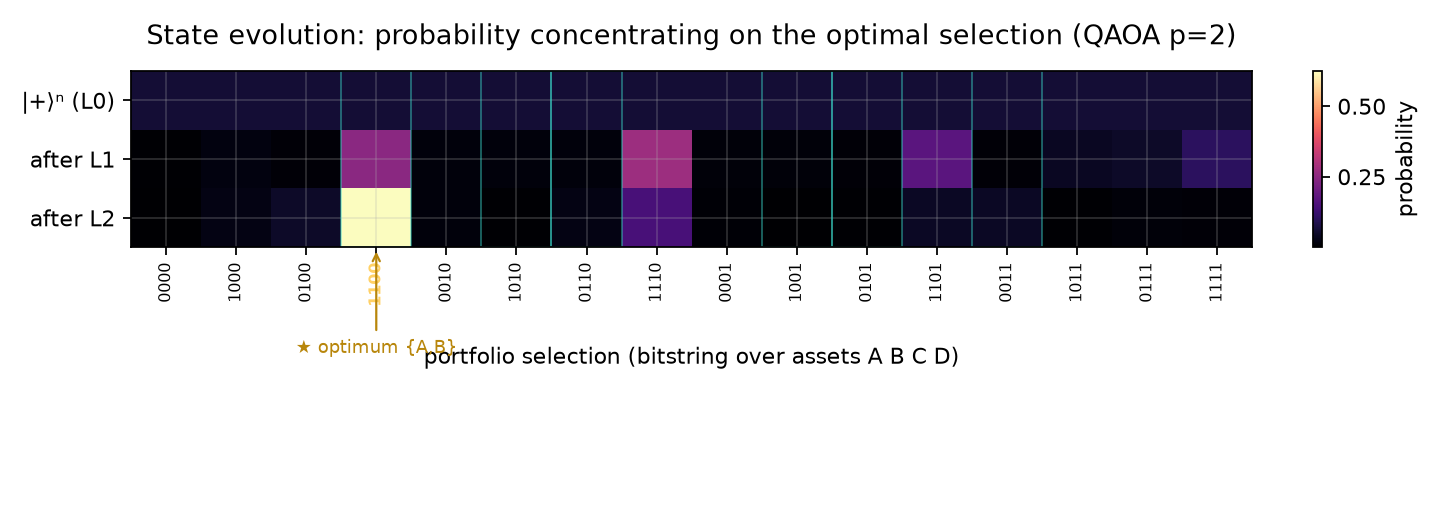
\includegraphics[width=\linewidth]{figures/fig1_state_evolution.png}
\caption{State evolution: probability over all $2^n$ candidate selections from the uniform superposition
(top row) onto the optimal feasible portfolio (starred) across QAOA layers.}
\label{fig:evo}
\end{figure}

\paragraph{The state concentrates on the optimum (Fig.~\ref{fig:evo}, Fig.~\ref{fig:depth}).}
On a well-separated 4-asset instance ($B{=}2$), the output evolves from uniform
(P(opt)$=\Puniform$, in three layers $0.062\!\to\!0.25\!\to\!\Popt$) to a sharp peak on the optimum at
depth $p{=}2$: P(opt)$=\Popt$ ($\Conc\times$ a uniform guess), approximation ratio $\AR$, with
best-sample recovery of the exact optimum. Depth $p{=}1$ is insufficient (AR $0.50$); $p{=}2$ already
cracks the instance, and $p{=}4$ sharpens it further (P(opt)$=\Poptd$, AR $\ARd$).

\begin{figure}[t]\centering
\begin{minipage}{0.49\linewidth}\centering
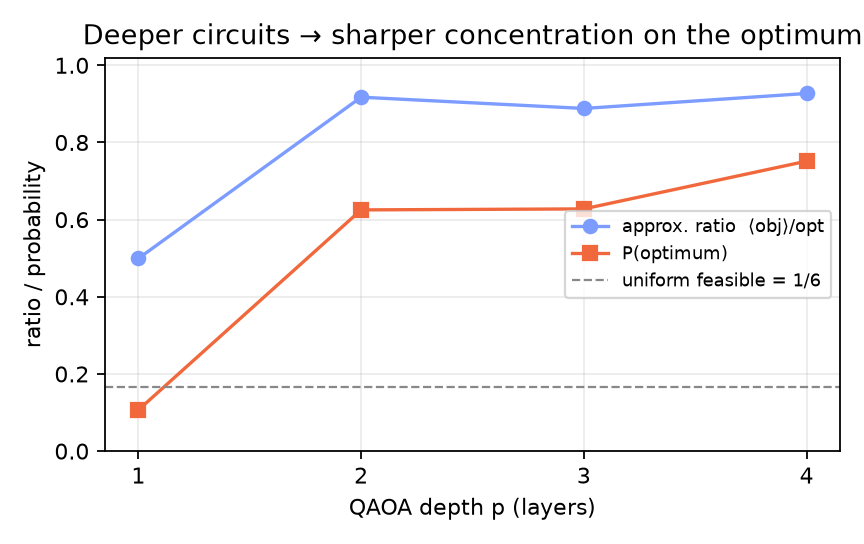
\includegraphics[width=\linewidth]{figures/fig2_depth.png}
\caption{Approximation ratio and P(optimum) rise with circuit depth.}\label{fig:depth}
\end{minipage}\hfill
\begin{minipage}{0.49\linewidth}\centering
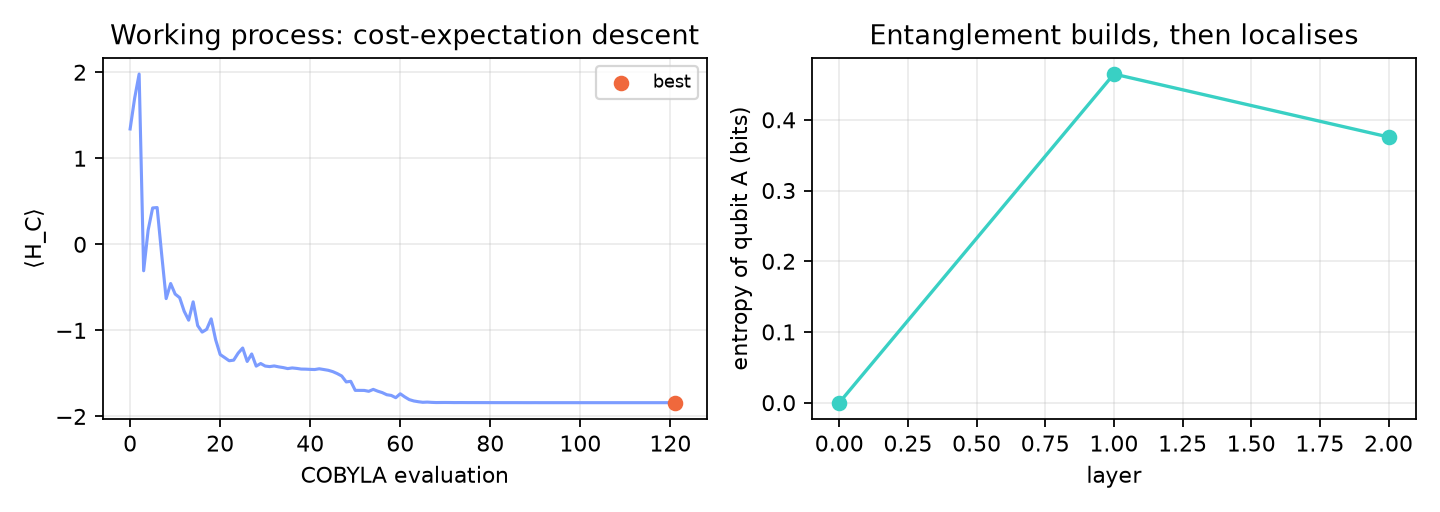
\includegraphics[width=\linewidth]{figures/fig3_process.png}
\caption{The working process: $\langle H_C\rangle$ descent and per-layer entanglement.}\label{fig:proc}
\end{minipage}
\end{figure}

\paragraph{Language steers the ground state (Fig.~\ref{fig:lang}).}
From the neutral optimum $\{A,B\}$, a rising LLM bullish view on $\{C,D\}$ migrates the exact optimum
$\{A,B\}\!\to\!\{A,C\}\!\to\!\{C,D\}$, and the QAOA \emph{modal selection tracks the language-shifted
optimum in all three regimes} (approximation ratios $0.92$/$0.92$/$0.85$). The selection is a continuous
function of language: weak conviction swaps one holding, strong conviction flips the book. Concentration
is naturally lower under a strong view ($P(\text{opt}){=}0.16$--$0.19$) because the tilt creates
near-ties among portfolios---an honest reflection of genuine ambiguity, not optimizer failure. To our
knowledge this is the first demonstration of a natural-language view visibly deforming the state
evolution of a quantum portfolio optimizer.

\begin{figure}[t]\centering
\begin{minipage}{0.55\linewidth}\centering
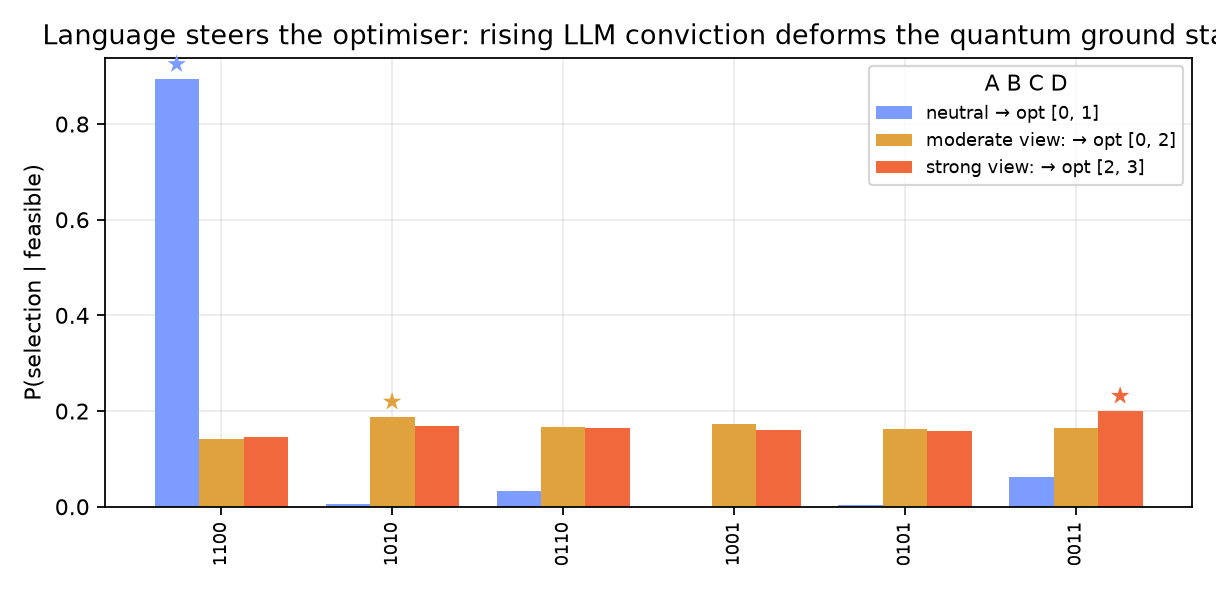
\includegraphics[width=\linewidth]{figures/fig4_language.png}
\caption{Rising LLM conviction deforms the quantum ground state across feasible portfolios.}
\label{fig:lang}
\end{minipage}\hfill
\begin{minipage}{0.43\linewidth}\centering
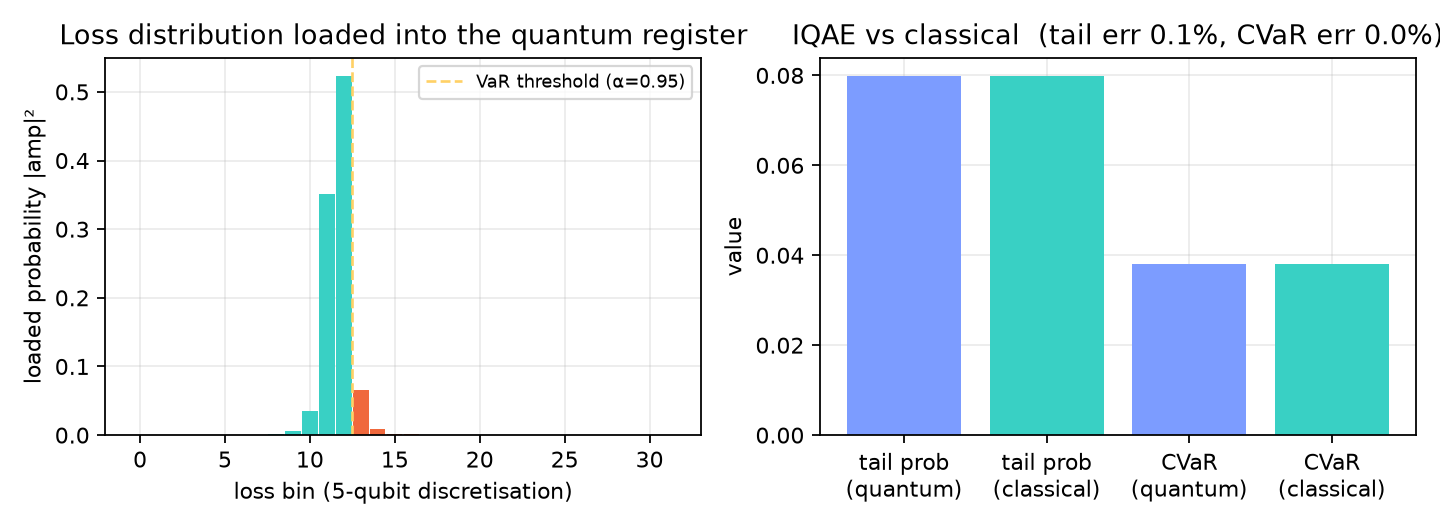
\includegraphics[width=\linewidth]{figures/fig5_risk.png}
\caption{IQAE loads the loss distribution and recovers tail/CVaR to within a few percent.}
\label{fig:risk}
\end{minipage}
\end{figure}

\paragraph{Risk replication (Fig.~\ref{fig:risk}).}
The IQAE circuit loads a fat-tailed (Student-$t$) loss onto 5 qubits at $\alpha{=}0.95$. The
quantum-estimated quantity is the tail-exceedance probability $P(\text{loss}\ge\text{VaR})$, which IQAE
recovers to within $\TailErr\%$ of the loaded distribution; CVaR then follows from that distribution.
This reproduces the Woerner--Egger primitive on our instance.

\section{Related Work and Limitations}
Our core is QAOA~\citep{farhi2014qaoa}; the CVaR-objective variational idea is~\citet{barkoutsos2020cvar};
the risk circuit replicates~\citet{woerner2019risk} with the IQAE estimator
of~\citet{grant2021iqae}, in the lineage of quantum option pricing~\citep{stamatopoulos2020option} and
the IBM survey~\citep{egger2020finance}. QNLP~\citep{coecke2010dispho,lorenz2023qnlp} motivates language
as a first-class quantum input; we differ by routing \emph{LLM-derived} views into a finance optimizer's
Hamiltonian and foregrounding \emph{visualization}.
\textbf{Limitations:} results are on small ($n{=}4$--$8$), well-separated, exactly-simulated instances;
we make no scaling or supremacy claim, brute force is our oracle, the language tilt is a simple additive
mechanism, and the IQAE advantage is asymptotic in $\varepsilon$, not a wall-clock speedup here.

\section{Conclusion}
Making a quantum optimizer's state evolution and working process visible---and showing language steer
it---offers an auditable template for high-stakes quantum finance and a concrete QNLP $\times$
quantum-optimization use case. Everything is reproducible from \texttt{python -m paper.experiments}.

\small
\bibliographystyle{plainnat}
\bibliography{references}
\end{document}
